%-------------------------------------------------------------------------------
%-------------------------------------------------------------------------------
\section{Valeurs et vecteurs propres, diagonalisation} \label{sec:LinAlg-Eigen}
%-------------------------------------------------------------------------------
%-------------------------------------------------------------------------------

%-------------------------------------------------------------------------------
%-------------------------------------------------------------------------------
\subsection{Valeurs et vecteurs propres} \label{sec:ValVecPropres}
%-------------------------------------------------------------------------------

\begin{definition*}[Valeur et vecteur propre]
  $\lambda \in \Rbb$ est une valeur propre de $A \in \Mcal_n(\Rbb)$ ssi, il existe un vecteur non nul $x \in \Rbb^n$ tel que $A x = \lambda x$. $x$ est appelé vecteur propre de $A$ associé à $\lambda$.
\end{definition*}

\begin{exercise*}
  Donner $n$ valeurs propres (et les vecteurs propres associés) de la matrice 
  $$
  D = \diag(\mu_1, \mu_2, \dots, \mu_n).
  $$
\end{exercise*}

\solution{Les $n$ vecteurs de la base canonique.}

\begin{proposition*}[Vecteur propre]
  Si $x$ est un vecteur de propre de $A$ associé à la valeur propre $\lambda$, $y = k x$ l'est également.
\end{proposition*}

\proof 
  C'est une conséquence de la linéarité de la multiplication de $x$ par $A$ : 
  $$
  A y = A \times (k x) = k (A \times x) = k (\lambda x) = \lambda (k x) = \lambda y.
  $$
%   $x$ est un vecteur de propre de $A$ associé à la valeur propre $\lambda$ ssi, pour tout $1 \leq i \leq n$, 
%   $$
%   \sum_{j=1}^n a_{ij} x_j = \lambda x_i.
%   $$
%   Si $y = a x$, alors pour tout $1 \leq i \leq n$, $y_i = b x_i$, et donc
%   $$
%   \sum_{j=1}^n a_{ij} y_j 
%   = \sum_{j=1}^n a_{ij} b x_j
%   = b \sum_{j=1}^n a_{ij} x_j
%   = b \lambda x_i
%   = \lambda y_i.
%   $$
\eproof

\remark
Parler ``du'' vecteur propre $x$ associé à la valeur propre $\lambda$ est donc un abus de langage. Tous les vecteurs engendrés par $x$ sont également propres : on peut aussi parler plus précisément de {\em direction propre}.

\begin{exercise*}
  Déterminer les valeurs propres de 
  $$
  A = \left[\begin{array}{rr} 1 & 1 \\ 3 & -1 \end{array}\right].
  $$
\end{exercise*}

\solution{
  On cherche $x = [x_1 \; x_2]$ tel que $Ax = \lambda x$, c'est-à-dire
  $$
  \left\{\begin{array}{rl}
    x_1 + x_2 & = \lambda x_1 \\
    3 x_1 - x_2 & = \lambda x_2 
  \end{array} \right\}
  \quad \Leftrightarrow \quad 
  \left\{\begin{array}{rl}
    x_2 & = (\lambda -1) x_1 \\
    3 x_1 - (\lambda - 1) x_1 & = \lambda (\lambda - 1) x_1
  \end{array} \right\}
  \quad \Leftrightarrow \quad 
  \left\{\begin{array}{rl}
    x_2 & = (\lambda -1) x_1 \\
    0 & = (\lambda ^2 - 4) x_1
  \end{array} \right\} 
  $$
  On remarque que $\{\lambda= 1\} \Rightarrow \{x_2 = 0, x_1 = 0\}$ et que $\{x_1 = 0, \lambda \neq 1\} \Rightarrow \{x_2 = 0\}$. Donc $\lambda \neq 1$ et $x_1 \neq 0$ (sinon la solution est le vecteur nul). $\lambda$ doit donc satisfaire  
  $$
  \lambda ^2 - 4 \qquad \Leftrightarrow \qquad \lambda \in \{-2, 2\}.
  $$
  On peut alors déterminer les vecteurs propres associés
  \begin{align*}
    \lambda & = -2 &
    \Rightarrow \; &
    \left\{\begin{array}{rl}
      x_1 + x_2 & = -2 x_1 \\
      3 x_1 - x_2 & = -2 x_2 
    \end{array} \right\} &
    \Rightarrow \; &
      x_2 = -3 x_1
    \qquad \text{soit, par exemple, } u_1 = \left[\begin{array}{r} 1 \\ -3 \end{array}\right], \\
    \lambda & = 2 &
    \Rightarrow \; &
    \left\{\begin{array}{rl}
      x_1 + x_2 & = 2 x_1 \\
      3 x_1 - x_2 & = 2 x_2 
    \end{array} \right\} &
    \Rightarrow \; &
      x_2 = x_1
    \qquad \text{soit, par exemple, } u_2 = \left[\begin{array}{r} 1 \\ 1 \end{array}\right]. 
  \end{align*}
}

\remark Les vecteurs et valeurs propres décrivent comment l'opérateur associé à la matrice $A$ agit sur un vecteur $x$ quelconque. 

%-------------------------------------------------------------------------------
\paragraph{Exemple.} Dans l'exemple de l'exercice, les vecteurs propres 
$$
u_1 = \left[\begin{array}{r} 1 \\ -3 \end{array}\right]
\qquad \text{et} \qquad 
u_2 = \left[\begin{array}{r} 1 \\ 1 \end{array}\right]
$$
sont linéairement indépendants, donc on peut décomposer tout vecteur $x \in \Rbb^2$ en
$$
x = c u_1 + d u_2.
$$
Par linéarité, on a 
$$
A x = c A u_1 + d A u_2 = c \lambda_1 u_1 + d \lambda_2 u_2 = -3 c u_1 + 2 d u_2.
$$
La composante de $x$ dans la direction de $u_1$ est multipliée par $\lambda_1 = -2$ et sa composante dans la direction de $u_2$ est multipliée par $\lambda_2 = 2$.

\dessin{Transformation des deux composantes du vecteur $x = u_1 + 2u_2$ : 
$$
x = u_1 + 2u_2 = \left[\begin{array}{r} 3 \\ -1 \end{array}\right]
\qquad \Rightarrow \qquad
Ax = -3 u_1 + 4 u_2 =  \left[\begin{array}{r} 2 \\ 10 \end{array}\right].
$$
}

\remark La détermination des valeurs et vecteurs propres est passée par la détermination des racines d'un polynôme.

%-------------------------------------------------------------------------------
%-------------------------------------------------------------------------------
\subsection{Polynôme caractéristique} \label{sec:polCarac}
%-------------------------------------------------------------------------------

\begin{definition*}[Polynôme caractéristique]
  Le polynôme caractéristique de la matrice $A \in \Mcal_n$ est l'application 
  $$
  \begin{array}{r|rcl}
   P_A: & \Rbb & \mapsto & \Rbb \\
    & \lambda & \rightarrow & |A - \lambda I_n|.
  \end{array}
  $$
\end{definition*}

\begin{exercise*}
  Déterminer le polynôme caractéristique de la matrice $A \in \Mcal_n$ diagonale de diagonale $(\mu_1, \dots, \mu_n)$.
\end{exercise*}

\solution{
  $$
  P_A(\lambda) = \prod_{i=1}^n (\mu_i - \lambda).
  $$
}

\begin{exercise*}
  Déterminer le polynôme caractéristique de la matrice
  $$
  A = \left[\begin{array}{rr} 1 & 1 \\ 3 & -1 \end{array}\right].
  $$
\end{exercise*}

\solution{$P_A(\lambda) = \lambda^2 - 4$.}


\begin{theorem*}
  $\lambda$ est une valeur propre de la matrice $A$ ssi $P_A(\lambda) = 0$.
\end{theorem*}

\proof
  \begin{align*}
    p_A(\lambda) = 0 
    & \quad \Leftrightarrow \quad |A - \lambda I| = 0 \\
    & \quad \Leftrightarrow \quad A - \lambda I \text{ pas inversible} \\
    & \quad \Leftrightarrow \quad \exists y: (A - \lambda I)x = y \text{ admet plusieurs solutions $x$} \\
    & \quad \Leftrightarrow \quad \exists y: (A - \lambda I)(x_1 - x_2) = y-y = 0 \text{ admet une solution $(x_1, x_2): x_1 \neq x_2$} \\
    & \quad \Leftrightarrow \quad \exists z \neq 0: (A - \lambda I)z = 0 \\
    & \quad \Leftrightarrow \quad \exists z \neq 0: A z = \lambda z \\
    & \quad \Leftrightarrow \quad \lambda \text{ valeur propre de } A. 
  \end{align*} 
\eproof

\begin{definition*}[Trace]
  La trace d'une matrice $A \in \Mcal_n$ est notée $\tr(A)$ et est égale à la somme de ses termes diagonaux :
  $$
  \tr(A) = \sum_{i=1}^n a_{ii}.
  $$
\end{definition*}


\begin{exercise*}[Ex 1.3.3 : Cas d'une matrice $2 \times 2$]
  On considère la matrice $A \in \Mcal_2$:
  $$
  A = \left[\begin{array}{cc} a & b \\ c & d\end{array}\right]
  $$
  Déterminer le polynôme caractéristique de $A$ et donner les condtions sur $p = \tr(A)$ et $q = \det(A)$ pour que $A$ admette deux valeurs propres réelles.
\end{exercise*}

\solution{
  On a 
  $$
  |A - \lambda I_2| 
  = \left|\begin{array}{cc} a - \lambda & b \\ c & d - \lambda \end{array}\right|
  = (a - \lambda)( d - \lambda) - bc
  = \lambda^2 - (a+d) \lambda + (ad - bc)
  = \lambda^2 - p \lambda + q
  $$
  qui admet deux solutions réelles (éventuellement égales) ssi
  $$
  p^2 - 4 q \geq 0
  \qquad \Leftrightarrow \qquad
  q \leq p^2 / 4.
  $$
  $$
  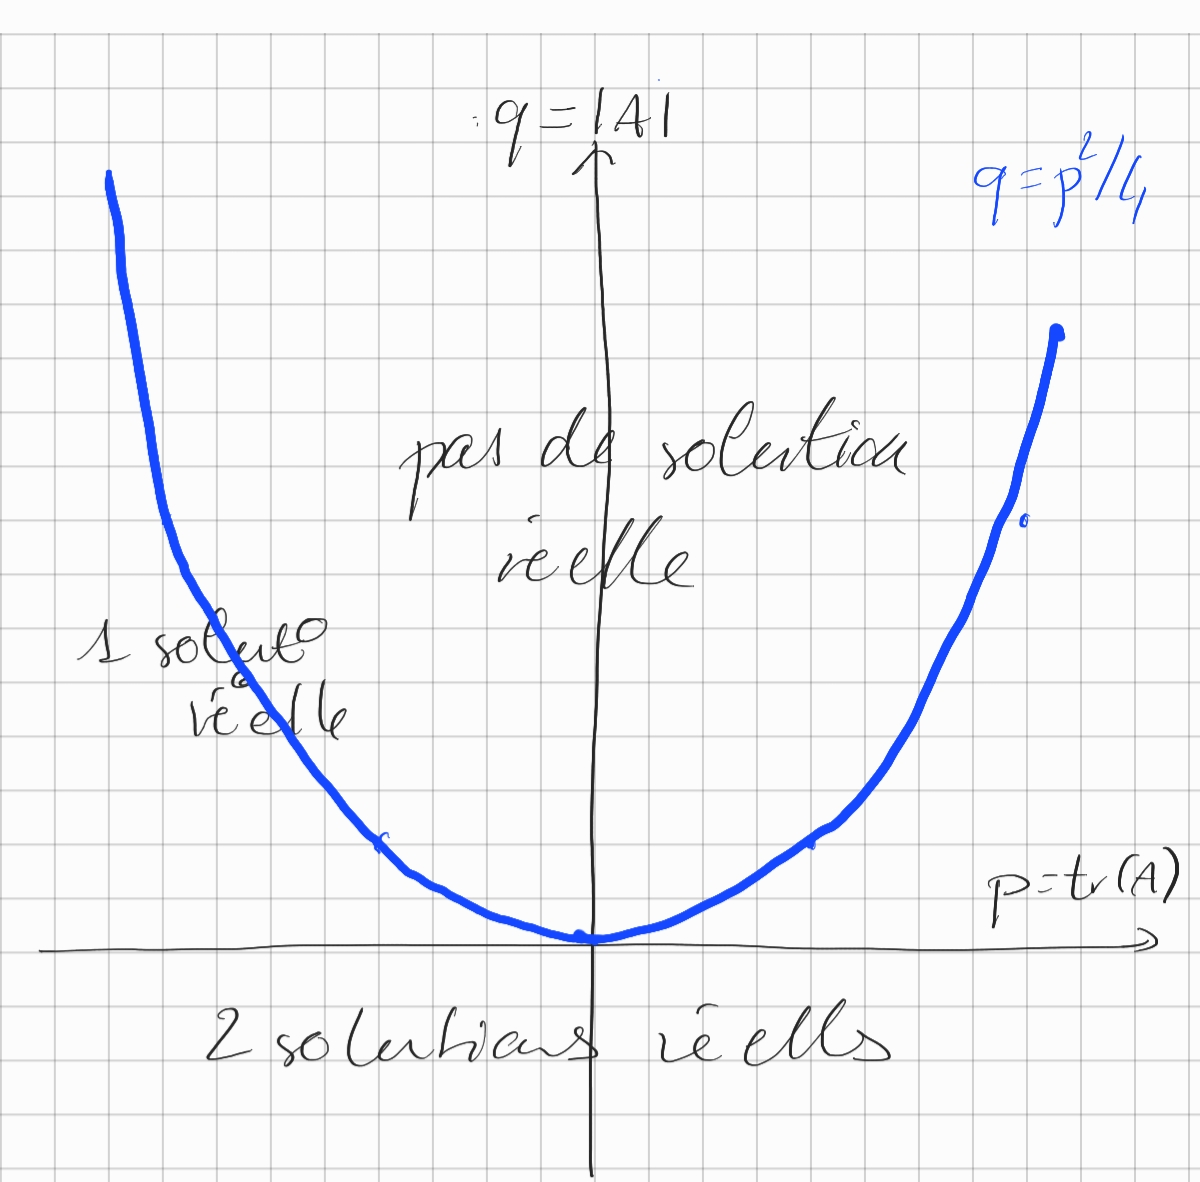
\includegraphics{ValeursPropresReellesDimension2} 
  $$
}

\begin{theorem*}[Propriétés du polynôme caractéristique]
  Le polynôme caractéristique $P_A$ de la matrice $A \in \Mcal_n(\Rbb)$ est de degré exactement $n$ et, en notant $[\lambda^k]P_A(\lambda)$ le coefficient d'ordre $k$ de $P_A(\lambda)$:
  $$
  [\lambda^n]P_A(\lambda) = (-1)^n, \qquad
  \textcolor{gray}{[\lambda^{n-1}]P_A(\lambda) = (-1)^{n-1} \tr(A), \qquad}
  [\lambda^0]P_A(\lambda) = \det(A).
  $$
\end{theorem*}

\proof
\begin{enumerate}[\itemdot]
 \item La propriété $[\lambda^0]P_A(\lambda) = \det(A)$ est immédiate en se remarquant que
$$
[\lambda^0]P_A(\lambda) = P_A(0) = |A - 0 I_n| = |A|.
$$
\item La formule \eqref{eq:determinant} montre que le degré de $P_A$ ne peut excéder $n$ puisque chaque permutation emprunte au plus $n$ termes diagonaux.
\item Les autres propriétés se montrent par récurrence en commençant par remarquer qu'elles sont toutes vraies pour $n = 2$ (cf Exercice 1.3.3). Pour la récurrence, on développe $|A - \lambda I_n|$ par rapport à la dernière ligne : 
$$
|A - \lambda I_n| 
= \sum_{j=1}^{n-1} a_{nj} \underset{\scriptsize
  \begin{tabular}{c}\text{degrée $\leq n-1$ par \eqref{eq:determinant}} \\
  \text{car aucune permutation n'emprunte} \\
  \text{2 fois la même ligne ou la même colonne}\end{tabular}
  }{\underbrace{|(A - \lambda I_n)^{(nj)}|}} + (a_{nn} - \lambda) \underset{\text{degrée $= n-1$ par hypothèse}}{\underbrace{|(A - \lambda I_n)^{(nn)}|}}
$$
Donc
$$
[\lambda^n]|A - \lambda I_n| 
= [\lambda^n](-\lambda |(A - \lambda I_n)^{(nn)}|) 
= - [\lambda^{n-1}]\underset{\text{$= (-1)^{n-1}$ par hypothèse}}{\underbrace{(|(A - \lambda I_n)^{(nn)}|)}}
= (-1)^n
$$
et le degré de $P_A$ est donc supérieur ou égal à $n$
\item \textcolor{gray}{La démonstration pour le coefficient d'ordre $n-1$ ($= [\lambda^{n-1}]P_A(\lambda)$) suit le même principe.}
\end{enumerate}
\eproof

\begin{corollary*}
  Le déterminant est égal au produit des valeurs propres : 
  $$
  |A| = \prod_{i=1}^d \lambda_i^{m_i}.
  $$
\end{corollary*}

\proof
  Il suffit de remarquer que, du fait des propriétés du polynôme caratéristique et de sa factorisation, 
  $$
  |A| = [\lambda^0]P_A(\lambda) = \prod_{i=1}^d \lambda_i^{m_i}.
  $$
\eproof

%-------------------------------------------------------------------------------
\subsubsection{Rappel sur les polynômes} 
%-------------------------------------------------------------------------------

\begin{proposition*}[Polynômes à coefficients réels]
  Tout polynôme à coefficients réels est scindé sur $\Cbb$, c'est à dire que, pour $P$ de degré exactement $n$, il existe un réel $a$ non nul et $n$ nombres complexes $x_1, \dots, x_n$ (non nécessairement distincts) tels que
  $$
  P(x) = a \prod_{i=1}^n (x_i - x).
  $$
  $x_1, \dots, x_n$ sont des racines de $P$.
\end{proposition*}

\proof
Non démontré
\eproof

\begin{definition*}[Ordre de multiplicité]
  On note $d$ le nombre de racines distinctes d'un polynôme $P$ de degré $n$ et $x_1, x_2, \dots x_d$ ces racines. On peut alors écrire $P$ sous la forme
  $$
  P(x) = a \prod_{j=1}^d (x_i - x)^{m_i}
  $$
  et $m_j$ est appelé ordre de multiplicité de la racine $x_j$ et les $m_j$ vérifient $ \sum_{j=1}^d m_j = n$.
\end{definition*}

%-------------------------------------------------------------------------------
\paragraph{Exemple.} 
$$
P(x) = x^3 - 4x^2 + 5x - 2 = (x-2)(x-1)^2 = - (2-x)(1-x)^2
$$ 
admet $x_1 = 1$ et $x_2 = 2$ pour racines avec $m_1 = 2$ et $m_2 = 1$.


\begin{corollary*}[Polynômes caractéristique]
  Le polynôme caractéristique $P_A$ d'une matrice réelle s'écrit
  $$
  P_A(\lambda) = \prod_{j=1}^d (\lambda_i - \lambda)^{m_i}
  $$
  où les $\lambda_i$ sont les $d$ valeurs propres distinctes de $A$.
\end{corollary*}

\proof
Les $\lambda_i$ sont les racines de $P_A$ et le coefficient $a$ vaut 1 puisque $[\lambda^n]P_A(\lambda) = (-1)^n$.
\eproof

%-------------------------------------------------------------------------------
\subsubsection{Sous-espaces propres} 
%-------------------------------------------------------------------------------

\begin{definition*}[Sous-espace propre]
  On appelle sous-espace propre associé à la valeur propre $\lambda$, l'ensemble des vecteurs propres associés à $\lambda$ :
  $$
  \text{sous-espace propre}(\lambda) = \{x \in \Rbb: Ax = \lambda x\},
  $$
  qui est aussi le noyau de $A - \lambda I$ : 
  $$
  \Ecal(\lambda) = \text{sous-espace propre}(\lambda) = \{x \in \Rbb: (A - \lambda I)x = 0\} = \ker(A - \lambda I).
  $$
\end{definition*}

\begin{proposition*}[Intersection des espaces propres]
  Soit deux valeurs propres distinctes $\lambda_1$ et $\lambda_2$ d'une matrice $A \in \Mcal_n(\Rbb)$:
  $$
  \text{sous-espace propre}(\lambda_1) \cap \text{sous-espace propre}(\lambda_2) = 0_n.
  $$
\end{proposition*}

\proof
Directe car $Ax = \lambda_1 x = \lambda_2 x$ avec $\lambda_1 \neq \lambda_2$ ssi $x = 0$.
\eproof


\begin{proposition*}[Dimension de l'espace propre]
  Pour toute matrice $A \in \Mcal_n(\Rbb)$ et pour chacune de ses valeurs propres, 
  $$
  \dim(\Ecal(\lambda_i)) \leq m_i.
  $$
\end{proposition*}

\proof
Non démontré
\eproof

\remark
On sait donc que les différentes valeurs propres sont associées à des sous-espaces propres qui engendrent un sous-espace de $\Rbb^n$, mais pas nécessairement $\Rbb^n$ tout entier. L'action d'un matrice $A$ dans chacun de ces sous-espaces est une simple homothétie.

\bigskip
\progres{Début Cours 3. Rappels :
\begin{enumerate}[\itemdot]
 \item Polynôme caractéristique $P_A$ : valeurs propres (réelles ou complexes) d'une matrice = racines de $P_A$ 
 \item $\det(A) = \prod_{i=1}^n \lambda_i = \prod_{j=1}^d \widetilde{\lambda}_j^{m_j}$
 \item Sous-espace propre $\Ecal(\lambda)$ associé à une val. propre $\lambda$ réelle
 \item Sous-espace propres disjoints : $\lambda_1 \neq \lambda_2 \Rightarrow \Ecal(\lambda_1) \cap \Ecal(\lambda_2) = \{0\}$
 \item Lien entre dimension de $\Ecal(\lambda_i)$ et ordre de multiplicité $m_i$
\end{enumerate}
}

%-------------------------------------------------------------------------------
%-------------------------------------------------------------------------------
\subsection{Matrices diagonalisables} \label{sec:MatDiag}
%-------------------------------------------------------------------------------

\begin{lemma*}
  L'inverse de la matrice diagonale $D = \diag(\mu_1, \dots \mu_n$) dont tous les termes diagonaux sont non nuls est la matrice diagonale $D^{-1} = \diag(\mu_1^{-1}, \dots \mu_n^{-1})$.
\end{lemma*}

\proof
On vérifie que $D D^{-1} = D^{-1} D = I_n$.
\eproof

\begin{definition*}[Matrice diagonalisable]
  Une matrice $A \in \Mcal_n(\Rbb)$ est dite diagonalisable s'il existe un matrice $D \in \Mcal_n(\Rbb)$ diagonale et une matrice $P \in \Mcal_n(\Rbb)$ inversible telles que
  $$
  A = P D P^{-1}
  $$
  et, en notant $D = \diag(d_1, \dots d_n)$ et $P = [u_1 \dots u_n]$, 
  $$
  \forall 1 \leq j \leq n: \quad A u_j = d_j u_j.
  $$
\end{definition*}

\remark
Une matrice $A$ est diagonalisable si son application consiste à
\begin{description}
 \item[$P^{-1}$:] Passer de la base canonique à la base constituée des vecteurs colonnes de $P$,
 \item[$D$:] Appliquer à chaque coordonnée de la nouvelle base une homothétie de rapport $d_i$,
 \item[$P$:] Revenir dans la base canonique.
\end{description}

\begin{proposition*}
  Les terme diagonaux de la matrice $D$ sont les valeurs propres de $A$ et les colonnes de la matrice $P$ sont les vecteurs propres associés.
\end{proposition*}

\proof
  On note $P = [u_1 \; u_2 \; \dots u_n]$ les colonnes de $P$ et on calcule tous les produits $A u_i$ simultanément : 
  $$
  A P = P D P^{-1} P = P D,
  $$
  il suffit de se rappeler que la multiplication à droit par une matrice diagonale multiple chaque colonne par le terme diagonal correspondant pour conclure que $P u_i = d_i u_i$ pour chaque $1 \leq i \leq n$.
\eproof

% \begin{proposition*}
%   Le déterminant d'une matrice diagonalisable est égal au produit de ses valeurs propres.
% \end{proposition*}

% \proof
% D'après la définition, les valeurs propres de $A$ sont les éléments diagonaux de la matrice $D$. On observe alors que
% $$
% |A| = |P D P^{-1}| = |P| |P^{-1}| |D| = |D| = \prod_i d_i.
% $$
% \eproof

\begin{proposition*}
  Si la matrice $A$ est diagonalisable ($A = P D P^{-1}$), son inverse vaut $A^{-1} = P D^{-1} P^{-1}$.
\end{proposition*}

\proof
On vérifie que $A A^{-1} = P D P^{-1} P D^{-1} P^{-1} = P D D^{-1} P^{-1} = P P^{-1} = I_n$ et idem dans l'autre sens.
\eproof

\begin{theorem*}[Théorème 1.3.8: Matrice diagonalisable]
  La matrice $A \in \Mcal_n(\Rbb)$ est diagonalisable ssi 
  \begin{enumerate}
   \item toutes ses valeurs propres $\lambda_i$ sont réelles et, 
   \item pour chacune d'elles, le sous-espace propre associé a pour dimension son ordre de multiplicité : 
   $$
   \dim(\Ecal(\lambda_i)) = m_i.
   $$
  \end{enumerate}
\end{theorem*}

\proof
Non démontré
\eproof

\begin{corollary*}
  Toute matrice $A \in \Mcal_n(\Rbb)$ dont les $n$ valeurs propres sont réelles et distinctes ($m_i = 1$, pour tout $i = 1 \dots n$) est diagonalisable.
\end{corollary*}

\proof
Tous les sous-espaces propres sont de dimension au moins 1 (puisqu'il existe un vecteur non nul tel que $Ax = \lambda_i x$). Comme la dimension d'un sous-espace propre ne peut pas excéder l'ordre de multiplicité, les deux valeurs coïncident et valent 1.
\eproof

\begin{corollary*}
  Si la matrice $A \in \Mcal_n(\Rbb)$ est diagonalisable, l'ensemble des sous-espace propres engendrent $\Rbb^n$ tout entier.
\end{corollary*}

\proof
C'est une conséquence de la proposition selon laquelle les intersections des sous-espapces propres sont réduites au vecteur nul.
\eproof

%-------------------------------------------------------------------------------
\paragraph{Exemple de matrices non diagonalisables.}
\begin{enumerate}
 \item Soit
 $$
 A = \left[\begin{array}{cc} 1 & 1 \\ 0 & 1 \end{array}\right],
 \qquad 
 P_A(\lambda) 
 = \left|\begin{array}{cc} 1-\lambda & 1 \\ 0 & 1-\lambda \end{array}\right|
 = (1 - \lambda)^2
 $$
 donc $\lambda_1 = 1$ est valeur propre d'ordre de multiplicité 2, mais
 $$
 Ax = \lambda_1 x \quad \Leftrightarrow \quad 
 \left\{\begin{array}{rcl} x_1 + x_2 & = & x_1 \\ x_2 & = & x_2 \end{array} \right. \quad \Leftrightarrow \quad 
 x_2 = 0
 \qquad (\text{soit } u_1 = e_1)
 $$
 donc le sous-espace propre associé est de dimension 1.
 \item Soit 
 $$
 A = \left[\begin{array}{rrr} 0 & 1 & 0 \\ 0 & 0 & 1 \\ 0 & 0 & 0 \end{array}\right],
 \qquad 
 P_A(\lambda) 
 = \left|\begin{array}{rrr} -\lambda & 1 & 0 \\ 0 & -\lambda & 1 \\ 0 & 0 & -\lambda \end{array}\right|
 = -\lambda^3
 $$
 donc $\lambda_1 = 0$ est valeur propre d'ordre de multiplicité 3, mais
 $$
 A x = \lambda_1 x \quad \Leftrightarrow \quad 
 \left\{\begin{array}{rcl} x_2 & = & 0 \\ x_3 & = & 0 \end{array} \right.
 $$
 donc le sous-espace propre associé est de dimension 1.
 \item Soit la matrice {\em circulante}
 $$
 A = \left[\begin{array}{rrr} 0 & 1 & 0 \\ 0 & 0 & 1 \\ 1 & 0 & 0 \end{array}\right],
 \qquad 
 P_A(\lambda) 
 = \left|\begin{array}{rrr} -\lambda & 1 & 0 \\ 0 & -\lambda & 1 \\ 1 & 0 & -\lambda \end{array}\right|
 = -\lambda^3 + 1
 $$
 qui s'annule pour 
 $$
 \lambda \in \left\{1, \frac{-1+i\sqrt{3}}{2}, \frac{-1-i\sqrt{3}}{2}, \right\}.
 $$
 Le sous-espace propre associé à $\lambda_1$ est dit {\em invariant} et correspond à la première bissectrice : 
 $$
 A x = \lambda_1 x \quad \Leftrightarrow \quad 
 \left\{\begin{array}{rcl} x_2 & = & x_1 \\ x_3 & = & x_2 \\ x_1 & = & x_3 \end{array} \right.
 $$
 L'action de $A$ dans les autres dimensions est une rotation.
\end{enumerate}

% \begin{exercise*}
%   Déterminer les polynômes caractéristiques des matrices suivantes et en déduire si elles sont diagonalisables ou non.
%   \begin{align*}
%     A_1 & = \left[\begin{array}{ccc}
%       2 & -1 & 3 \\ 2 & -1 & 6 \\ 1 & 0  & 2
%       \end{array}\right], &
%     A_2 & = \left[\begin{array}{ccc}
%       1 & 1 & 0 \\ -5 & -2 & 5 \\ -1 & 0 & 2
%       \end{array}\right], \\ 
%     %
%     A_3 & = \left[\begin{array}{ccc}
%       -1 & 3 & 1 \\ 0 & 2 & 1 \\ 0 & 3 & 0
%       \end{array}\right], & 
%     A_4 & = \left[\begin{array}{ccc}
%       -1 & 3 & 1 \\ 0 & 2 & 1 \\ \alpha & \beta & 2
%       \end{array}\right],  
%   \end{align*}
% \end{exercise*}

\begin{exercise*}
  Déterminer le polynôme caractéristique de la matrice
  $$
  A = \left[\begin{array}{rrr}
  -1 & 3 & 1 \\ 0 & 2 & 1 \\ 0 & 3 & 0
  \end{array}\right], 
  $$
  et en déduire si elle est diagonalisable ou non.
\end{exercise*}

\solution{
  $$
  P_A(\lambda) 
  = \left|\begin{array}{rrr}
    -1-\lambda & 3 & 1 \\ 0 & 2-\lambda & 1 \\ 0 & 3 & -\lambda
      \end{array}\right|
  = (-1 - \lambda)(-\lambda (2 - \lambda) - 3)
  % = -(1 + \lambda)(\lambda^2 - 2\lambda - 3)
  = -(1 + \lambda)^2(\lambda - 3)
  $$
  donc les valeurs propres sont $\lambda_1 = -1$ et $\lambda_2 = 3$ avec $m_1 = 2$, $m_2 = 1$ et
  $$
  Ax = -x \quad\Leftrightarrow \quad 
  \left\{\begin{array}{rcl}
    -x_1 + 3x_2 + x_3 & = & -x_1 \\
    2x_2 + x_3 & = & -x_2 \\
    3x_2 & = & -x_3 \\
  \end{array}\right. \quad\Leftrightarrow \quad 
  3x_2 = -x_3
  $$
  donc $\dim(\Ecal(\lambda_1)) = 2 = m_1$ et $A$ est donc diagonalisable.

  Deux vecteurs propres (indépendants) associés à $\lambda_1$ sont
  $$
  [0 \; 1 \; -3]^\top \qquad \text{et} \qquad [1 \; 1 \; -3]^\top 
  $$
  et un vecteur propre associé à $\lambda_2$ est 
  $$
  [1 \; 1 \; 1]^\top.
  $$
  On peut diagonaliser $A = P D P^{-1}$ avec
  $$
  D = \left[\begin{array}{rrr}
  -1 & 0 & 0 \\ 0 & -1 & 0 \\ 0 & 0 & 3
  \end{array}\right]
  \qquad \text{et} \qquad 
  P = \left[\begin{array}{rrr}
  0 & 1 & 1 \\ 1 & 1 & 1 \\ -3 & -3 & 1
  \end{array}\right].
  $$
}

\begin{theorem*}[Matrices réelles symétriques]
  Toute matrice $A \in \Mcal_n(\Rbb)$ symétrique ($A = A^\top$) est diagonalisable et ses vecteurs propres sont orthogonaux. 
\end{theorem*}

\proof
Non démontrée (programme de classe prépa BCPST). \\
% Voir Fre14-Notes-SymmetricMatricesAndEigendecomposition, section2, propositions 3 et 4.
\begin{itemize}
  \item Valeurs propres réelles : Le polynôme caratéristique de $A$ admet au plus $n$ racines éventuellement multiples et complexes. Si $\lambda$ est une valeur propre de $A$, en notant $\overline{\lambda}$ le conjugué de $\lambda$ ($\overline{\lambda} = \lambda \Leftrightarrow \lambda \in \Rbb$), il existe un vecteur $x$ tel que
  \begin{align*}
    Ax & = \lambda x & 
    \Rightarrow \qquad \overline{Ax} & = \overline{\lambda x} &
    \Rightarrow \qquad A \overline{x} & = \overline{\lambda} \overline{x} \\
    \Rightarrow \qquad x^\top A \overline{x} & = \overline{\lambda} x^\top \overline{x}
  \end{align*}
  puisque $A$ est réelle et que $\overline{a b} = \overline{a} \overline{b}$. De même on a
  \begin{align*}
    Ax & = \lambda x & 
    \Rightarrow \qquad \overline{x}^\top A x & = \lambda \overline{x}^\top x
    \Rightarrow \qquad x^\top A \overline{x} & = \lambda \overline{x}^\top x
  \end{align*}
  puisque $A$ est symétrique.
  \item \todo{}
\end{itemize}
\eproof
